\section{Our Approach}

\subsection{Pig Latin Features}
\begin{frame}{Features}
\begin{itemize}
	\item DataFlow Language:
	\begin{itemize}
		\item Programmer defines a sequence of statements where each carries out a single 					  data transformation. The output relation of each statement is stored in an  					  identifier to be used later in the program.
	\end{itemize}
	\item User Defined Functions:
	\begin{itemize}
		\item User defined functions provide the flexibility to perform specialized data 				 	  processing tasks.
	\end{itemize}
	\item Abstract Parallelism:
	\begin{itemize}
		\item Pig Latin programs are represented a sequential way to define the query 					      statements abstracting away the underlying parallelism performed through the 					  map-reduce tasks.
	\end{itemize}
\end{itemize}
\end{frame}

\subsection{Formalism}
\begin{frame}{Four Stages of Pig Programs}
\begin{itemize}
	\item A Pig Latin program passes through four stages of compilation:
	\begin{itemize}
		\item Pig Latin Program
		\item Logical Plan
		\item Physical Plan
		\item Map Reduce Phase
	\end{itemize}
	\item The logical plan is an one-to-one mapping from Pig Latin Program and the in Map-				  Reduces phase is executed by assigning physical operators to corresponding map-				  reduce jobs. So we've started our formalism by defining the calculus for Logical 				  plan and Map-Reduce in terms of Pig Latin programs.
\end{itemize}
\end{frame}

\subsection{Formalism for Logical Plan}

\begin{frame}{Conventions}
\centering
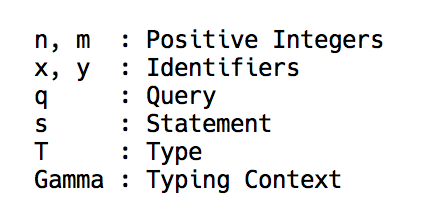
\includegraphics[scale=0.80]{conventions}
\end{frame}

\begin{frame}{Grammar: Queries}
\centering
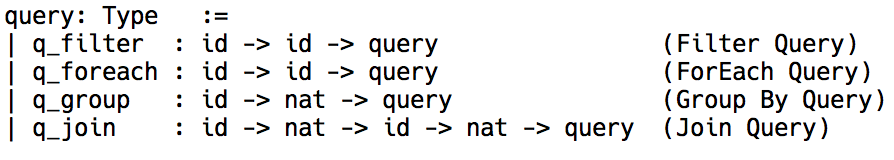
\includegraphics[scale=0.60]{query}
\end{frame}

\begin{frame}{Grammar: Statements}
\centering
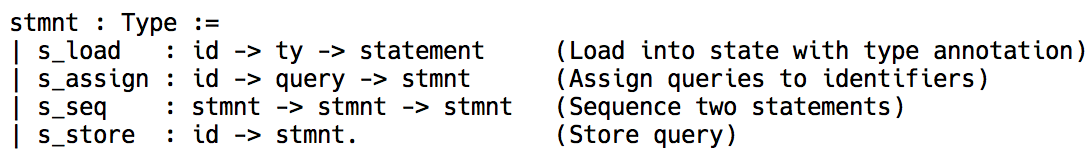
\includegraphics[scale=0.60]{stmnt}
\end{frame}

\begin{frame}{Types}
\centering
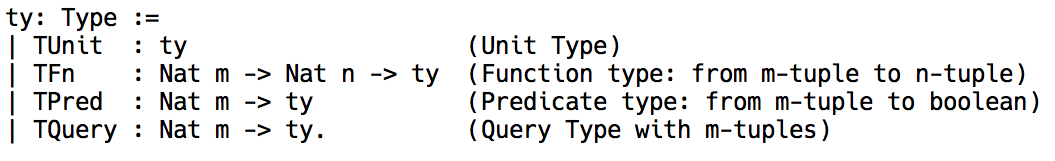
\includegraphics[scale=0.60]{ty}
\end{frame}

\begin{frame}{Typing Rules: Queries}
\centering
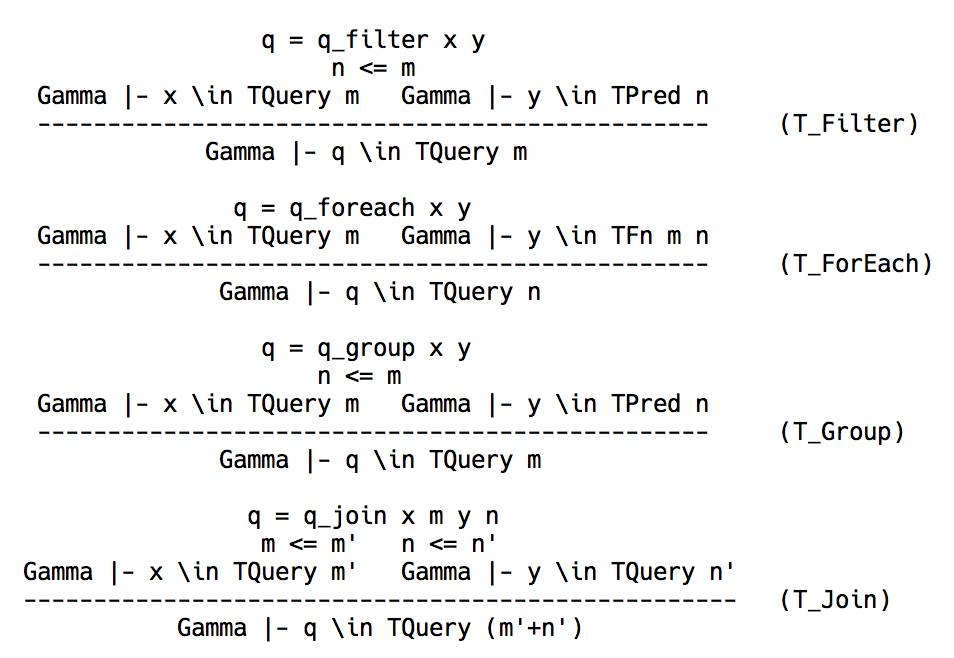
\includegraphics[scale=0.50]{T_Queries}
\end{frame}

\begin{frame}{Typing Rules: Statements}
\centering
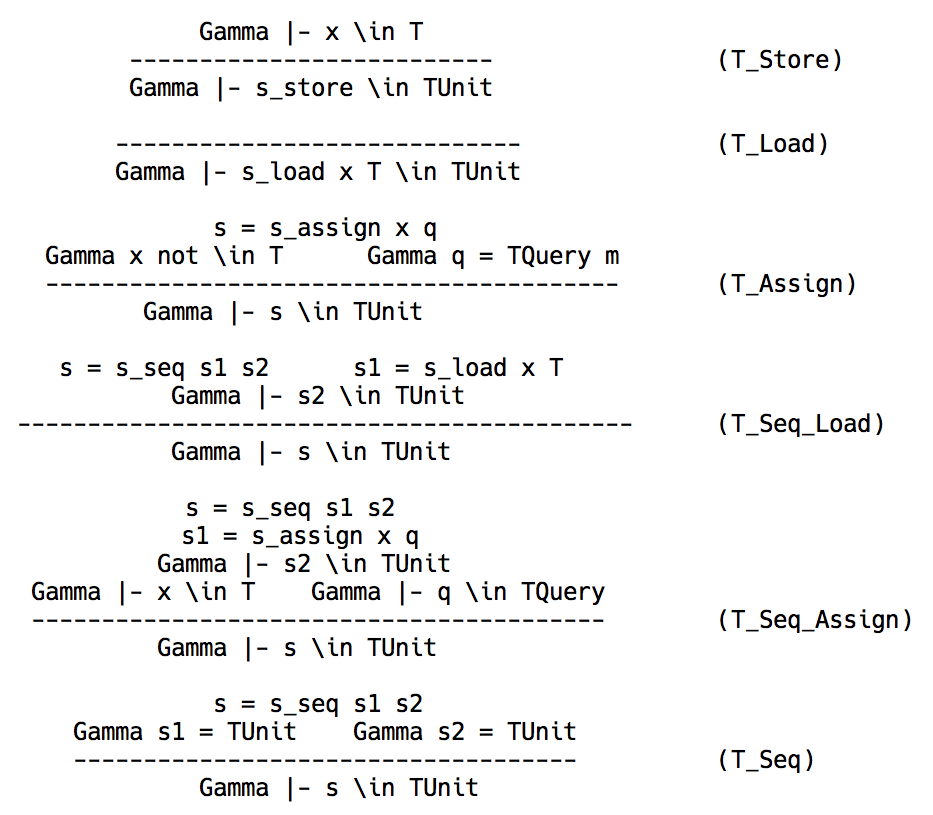
\includegraphics[scale=0.40]{T_Statements}
\end{frame}
